\documentclass{article}
\usepackage{graphicx} % Required for inserting images
\usepackage{amsmath}
\usepackage[numbers]{natbib}
\usepackage{url}
\usepackage{float}
\usepackage{etoolbox}
\usepackage{microtype}
\usepackage{placeins}
\setlength{\emergencystretch}{2em}
\AtBeginEnvironment{thebibliography}{\raggedright\sloppy}

\title{Beyond Geometric Heuristics: A Physics-Grounded Agent for\\
Self-Correcting Adsorption Configuration Discovery on Heterogeneous\\
Catalyst Surfaces}

\author{
Zongmin Zhang$^{1}$\thanks{Z.Z. is an undergraduate exchange student from the Hong Kong University of Science and Technology (HKUST),\\
participating in the official HKUST--EPFL exchange program, during which he conducted a semester-long research project at LIAC, EPFL.},
Junwu Chen$^{1}$,
Ryo Kuroki$^{1}$,\\
Xuan Vu Nguyen$^{1}$,\\
Edvin Fako$^{1\dagger}$,
Philippe Schwaller$^{1\dagger}$
}
% Author order is alphabetical among co-authors for this draft version, excluding the first author and PIs.

\date{26 February 2026}

\begin{document}

\begingroup\sloppy
\maketitle
\endgroup

\begin{center}
$^{1}$Laboratory of Artificial Chemical Intelligence (LIAC), EPFL,\\
Lausanne, Switzerland\\
$\dagger$Corresponding authors:

philippe.schwaller@epfl.ch

edvin.fako@epfl.ch
\end{center}

\begin{abstract}
The rational design of heterogeneous catalysts requires precise atomistic resolution of adsorbate configurations. However, on structurally complex multi-metallic surfaces, traditional discrete geometric heuristics fail, and exhaustive density functional theory (DFT) sampling remains computationally prohibitive. While large language models (LLMs) offer remarkable scientific reasoning capabilities, they suffer from a critical cognitive-physical gap when applied to complex interfaces, frequently hallucinating physically unstable binding sites due to intrinsic training data biases. Here, we introduce AdsMind, a physics-grounded autonomous scientific agent that operates as a closed-loop cognitive state machine for autonomous adsorption configuration discovery on heterogeneous catalyst surfaces. By seamlessly integrating a robust Surrogate SMILES translation layer with the rapid, high-fidelity physical verification via the MACE-MP machine learning force field, the agent iteratively generates, evaluates, and refines structural hypotheses. By offloading spatial deduplication to this active physical validation loop, the agent circumvents the severe $O(N^2)$ combinatorial bottleneck of traditional geometric symmetry reduction. Crucially, AdsMind explicitly tracks ``Chemical Slips''---spontaneous adsorbate migrations during relaxation, and updates its epistemic belief state via semantic negative constraints. Across a comprehensive 20-surface benchmark, the agent consistently outperformed static zero-shot LLM baselines, achieving a consistent success rate in navigating away from kinetically unstable initial guesses and converging to the putative global thermodynamic minimum within an average of 3.4 iterations. Furthermore, the agent incorporates an autonomous termination mechanism, proactively halting exploration upon detecting geometric convergence to a known historical best, thereby drastically reducing redundant compute cycles.Moreover, embedded topological analysis enabled the autonomous discovery of complex reactive events, including spontaneous dissociation and non-intuitive asymmetric multi-center coordination (e.g., 4-fold hollow sites on Cu-Zn oxide). By demonstrating that continuous physical feedback effectively de-biases frontier LLMs, AdsMind represents a critical paradigm shift from brute-force screening toward reasoning-driven, self-correcting autonomous discovery in computational catalysis.
\end{abstract}

\section{Introduction}
The rational design of heterogeneous catalysts critically depends on accurately resolving the atomistic configurations of adsorbates on structurally complex surfaces. This problem poses a severe combinatorial challenge, particularly for high-entropy alloys (HEAs) and amorphous materials, where catalytically active sites are neither well-defined nor readily identifiable, and consequently, the notion of discrete, symmetry-defined adsorption sites progressively breaks down. Although Density Functional Theory (DFT) offers a reliable physical reference, its prohibitive computational cost precludes exhaustive sampling of the vast chemical space. In contrast, conventional geometry-based heuristics provide computational efficiency but fail to explicitly capture the subtle electronic effects that govern adsorption phenomena on multi-metallic surfaces.

Recently, large language models (LLMs) have demonstrated remarkable potential in scientific reasoning tasks. Pioneering frameworks such as Adsorb-Agent~\cite{ock2024adsorbagent} have shown that LLMs can leverage their embedded chemical knowledge to substantially narrow the search space of adsorption configurations on heterogeneous catalyst surfaces. However, these first-generation agents predominantly operate in an open-loop manner, relying on the static prior knowledge encoded in the underlying model weights when selecting candidate adsorption sites. Recent benchmarks, including SUPERChem~\cite{zhao2025superchem}, have further revealed that even frontier LLMs struggle with complex, multi-step, constraint-aware chemical reasoning. Consistent with these observations, our systematic evaluation of 10 state-of-the-art (SOTA) foundation models from multiple providers (including OpenAI's GPT-5.2, Google's Gemini-3.1-Pro-Preview, Anthropic's Claude-Sonnet-4.6, and DeepSeek's DeepSeek-V3.2, among others. See Supplementary Table 1 for the full list) demonstrates that directly applying LLMs to structurally complex surfaces exposes an even more critical cognitive-physical gap (see Supplementary Table 1). Even advanced models suffer from pronounced training data biases (e.g., a rigid and systematic preference for Pd sites in atomic hydrogen adsorption) and are prone to hallucinations that result in frequently generating physically implausible geometries. In the absence of a closed-loop mechanism to ground and update hypotheses against post-relaxation physical feedback, static planning agents remain fundamentally constrained by the intrinsic limitations of their underlying models, regardless of scale.

To bridge this gap, we introduce AdsMind, a physics-grounded autonomous scientific agent capable of self-correcting discovery of the globally most stable adsorption configuration on heterogeneous catalyst surfaces. Unlike previous approaches that focus primarily on sampling efficiency, AdsMind operates as a cognitive state machine that iteratively generates, validates, and refines hypotheses, while explicitly updating its internal belief state based on physical feedback from structural relaxation. This architecture effectively couples the semantic reasoning of LLMs with the physical rigor of the MACE machine learning force field (MLFF). Furthermore, by integrating the AutoAdsorbate library~\cite{fako2025simple} as a geometry engine, our framework ensures robust and chemically valid conformer generation, going beyond the limitations of standard embedding techniques.

Our approach introduces three methodological innovations that distinguish it from existing pipelines:

\begin{enumerate}
    \item \textbf{Semantic-to-Geometric Projection:} We integrate a robust Surrogate SMILES translation layer, originally introduced by Fako \textit{et al.}~\cite{fako2025simple}, which enables the agent to project 1D chemical strings into 3D space. By employing surrogate atom(s) to orient the adsorbate relative to the surface normal, the agent effectively solves the adsorbate-interface alignment problem that plagues standard conformer embedding tools.
    \item \textbf{Self-Correcting Feedback Loop:} The agent moves beyond one-shot generation by actively analyzing structural relaxation results. By detecting the ``Chemical Slip'' phenomenon—where the adsorbate spontaneously migrates from the planned site to a distinct local minimum—the agent updates its internal belief state, allowing explicit recognition and correction of failures in its initial intuition and enabling convergence to configurations that defy simple geometric heuristics.
    \item \textbf{Handling Chemical Complexity:} The agent is engineered to detect and rationalize unusual phenomena such as spontaneous dissociation and on-surface isomerization, revealing the thermodynamic landscape often obscured by static geometric analysis.
\end{enumerate}

We benchmark AdsMind across 20 different surface environments, adopting the evaluation protocol established by Ock \textit{et al.}~\cite{ock2024adsorbagent} to ensure rigorous comparability (see Supplementary Table 2). Compared with static geometric enumeration baselines, the agent exhibits consistent convergence across multiple reasoning-relaxation cycles. In particular, in a supplementary stress test that involves adsorption of the formyl radical on a structurally complex Cu-Zn oxide surface, AdsMind identifies multiple energetically degenerate $\text{Cu}_{4}$ hollow sites among the lowest-energy configurations. By explicitly mapping exploration trajectories, AdsMind functions not merely as a global adsorption configuration optimizer but as an AI co-scientist that reveals a preliminary potential energy surface (PES) landscape for human experts and produces curated candidates for targeted DFT validation.

\section{Architecture}

\begin{figure}[htbp]
    \centering
    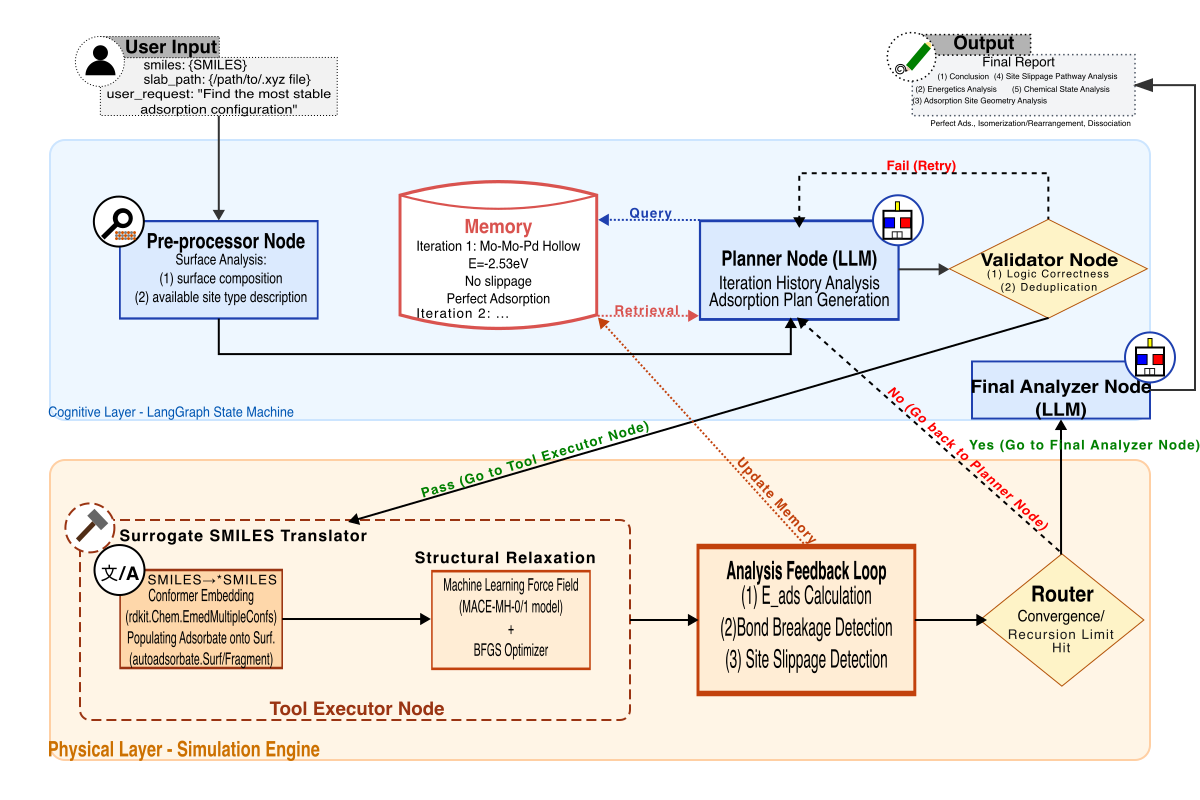
\includegraphics[width=1.0\textwidth]{images/workflow.png} 
    \caption{\textbf{The Cognitive State Machine Architecture of AdsMind.} The agent operates through a closed loop of planning, validation, execution, and analysis, explicitly bridging the gap between LLM reasoning and physical verification.}
    \label{fig:workflow}
\end{figure}

\FloatBarrier

\subsection{Cognitive Layer: Cognitive State Machine}
The cognitive layer orchestrates the autonomous discovery process by operating as a dynamic state machine designed to systematically reduce epistemic uncertainty. Unlike traditional high-throughput screening pipelines that blindly execute predefined spatial grids, AdsMind maintains a persistent, explicitly structured episodic memory of its exploration trajectory. The agent's internal belief state is represented as a continuously updating semantic map of geometric hypotheses, categorizing specific local surface domains as either viable targets or kinetically unstable regions.

The routing logic of the state machine is strictly governed by physics-derived triggers rather than stochastic resampling. Following each generation cycle, the agent evaluates the post-relaxation structural feedback. If the underlying physics engine reports ``Chemical Slip'' indicating that the adsorbate spontaneously migrated away from the semantically intended active site, the agent routes to a ``Correction and Refinement'' state. During this transition, the belief state undergoes a monotonic update: the failed geometric intent is formally eliminated from the viable hypothesis space via explicit negative constraints. This closed-loop epistemic update ensures that subsequent iterations are conceptually de-biased, autonomously driving the agent toward the thermodynamic sink without redundant exploration.

\subsection{Physics Layer: Physics-Informed Tools}
The physics layer serves as the rigorous verification environment, functioning as a bidirectional translation interface between the cognitive layer's semantic reasoning and the atomistic reality of the potential energy surface (PES). This layer executes a precise relay across three specialized operational domains.

Initially, the reasoning engine articulates a structural hypothesis as a purely semantic intent (e.g., targeting a specific multi-metallic bridge or hollow site). The geometry engine subsequently leverages the Surrogate SMILES translation layer to project this 1D semantic directive into a chemically valid 3D conformer, systematically resolving complex spatial and orientational constraints to instantiate the hypothesis on the slab model. Finally, the physics engine performs high-fidelity structural relaxation on this initial geometry.

Crucially, the feedback provided by the physics layer transcends simple scalar energy evaluations. The system actively analyzes the relaxation trajectory and inversely translates the final MLFF-relaxed atomic coordinates back into structured, semantic topological feedback. It autonomously categorizes the physical outcome by identifying the actual coordinated surface elements, detecting reactive events such as dissociation or isomerization, and explicitly quantifying site displacement. This rich, structured physical feedback is then seamlessly relayed back to the cognitive layer, directly informing the next cycle of hypothesis generation and belief updates.

\section{Methods}
\subsection{Semantic-to-Geometric Projection}
The translation of 1D semantic adsorption plans into collision-free 3D manifolds relies on a fortified Surrogate SMILES translation layer. To ensure robust structure generation across diverse and highly strained chemical spaces, the framework implements a cascading fallback protocol (ETKDGv3 $\rightarrow$ ETKDGv2 $\rightarrow$ Random Coordinates)~\cite{riniker2015better}. This is seamlessly coupled with a universal force field (UFF) pre-optimization step, which is dynamically bypassed for charged species to prevent classical force field failures.

Standard cheminformatics toolkits like RDKit enforce strict valence rules that frequently fail when handling radical species or multi-center coordination bonds on surfaces. AdsMind bypasses this using an electronic-state-aware bonding strategy. For targeted adsorbate atoms with unpaired radical electrons, covalent single bonds (\texttt{SINGLE}) are assigned to proxy atoms to reflect chemisorption physics. Conversely, for saturated atoms or lone pairs (e.g., carbonyl oxygen), dative bonds (\texttt{DATIVE}) are explicitly utilized to prevent valence over-saturation. For multi-point bridging or hollow sites, a dummy dimer proxy is employed, with its internal vector deterministically constrained based on the intended side-on or end-on vertical orientation.

Crucially, standard conformer embedding tools rely on strict symmetry reduction algorithms (\texttt{sym\_reduce}) to deduplicate topologically identical sites. However, on structurally complex multi-metallic surfaces lacking translational symmetry, these $O(N^2)$ distance-matrix comparisons introduce severe computational bottlenecks. Consequently, AdsMind deliberately bypasses geometric symmetry reduction. Instead, it employs a highly efficient capped random sampling strategy by evaluating a maximum of 8 spatial coordinates per semantic site type. While this introduces a minor risk of spatial clustering, it effectively trades exhaustive geometric coverage for a massive reduction in computational overhead, relying on the agent's iterative multi-start capability and active physical relaxation to ensure global exploration and deduplication. 

To ensure robust autonomous execution, the agent synergistically couples the LLM's high-dimensional semantic planning with meticulously pre-defined physical heuristics encoded in the geometry engine. For instance, while the physical engine autonomously determines atomic valency via RDKit radical counts, forcing the LLM to explicitly categorize the adsorbate type within its generation schema acts as a crucial ``cognitive scaffolding'', significantly reducing initial geometric hallucinations. The base surface-scanning algorithms were fundamentally fortified. The initial grid generation precision was doubled to 0.25 \AA{}, and the contact point detection tolerance ($\epsilon$) was expanded to 0.3 to prevent site omission on highly rugged topologies. Furthermore, the algorithm is constrained by a strict Z-axis penetration limit ($-1.0$ \AA{}) to prevent infinite-loop crashes within deep surface voids. Adsorbates targeting multi-coordination environments receive an automated $+0.5$ \AA{} pre-lift along the Cartesian Z-axis. To handle structural overlaps, a single-step Z-axis heuristic lift is applied to mitigate major initial steric clashes, while the subsequent $f_{max}$ filtering during pre-optimization effectively eliminates any residual physically implausible configurations. To eliminate spurious lateral self-interactions under periodic boundary conditions (PBCs), the agent automatically expands any primitive unit cell with insufficient lattice parameters into a larger supercell, while monitoring and alerting the user to potential spurious periodic interactions when the vacuum layer along the Z-axis is insufficient.

\subsection{Cognitive Machine and Self-Correcting Feedback Loop}
The search process is driven by an explicit epistemic update mechanism. Unlike static screening, AdsMind maintains a \textit{Semantic Spatial Memory} of all previous iterations. A ``Chemical Slip'' is rigorously defined as a divergence between the planned binding site and the post-relaxation geometric reality. The local bonding environment is reconstructed using element-specific natural cutoffs with a dynamic tolerance multiplier ($\alpha = 1.30$, extending to $1.45$ for strong chemisorption where $E_{ads} < -0.5$ eV).

The search process is driven by an explicit epistemic update mechanism. Unlike static screening, AdsMind maintains a \textit{Semantic Spatial Memory} of all previous iterations. A ``Chemical Slip'' is rigorously defined at the elemental level. It is triggered exclusively when the set of element symbols of the actually coordinated surface atoms post-relaxation strongly deviates from the LLM's planned binding symbols, rather than relying on ambiguous spatial displacements. The local bonding environment is reconstructed using element-specific natural cutoffs with a dynamic tolerance multiplier ($\alpha = 1.30$, extending to $1.45$ for strong chemisorption where $E_{ads} < -0.5$ eV).

When a slip or thermodynamic instability is detected, the analyzer injects a rigid negative feedback directive (the \texttt{FORBID} constraint) into the LLM’s history log. This forces the agent to eliminate kinetically unstable regions from its hypothesis space, dynamically guiding the search toward the putative thermodynamic minimum within a maximum limit of 5 iterations. Crucially, the agent is not merely bounded by this static limit. It incorporates an active autonomous termination mechanism. Upon detecting that a post-relaxation geometry matches a known historical best in both energetic and crystallographic fingerprints tagged via a specific `[Converged to known best]` semantic flag, the cognitive state machine autonomously issues a termination directive, prematurely halting the loop to conserve computational resources.

\begin{figure}[H]
    \centering
    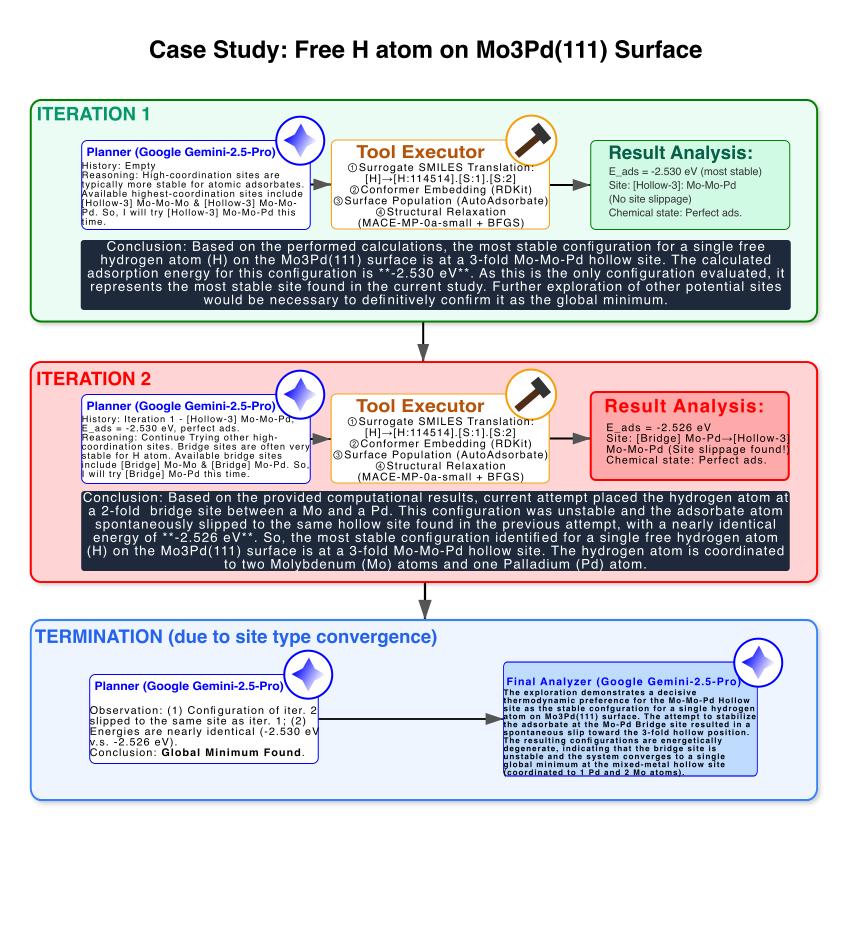
\includegraphics[width=1.0\textwidth]{images/demo.png}
    \caption{\textbf{Step-by-Step Execution Trace of the Self-Correcting Mechanism.}
    A detailed case study of atomic hydrogen (H) adsorption on the $\text{Mo}_{3}\text{Pd}(111)$ surface.
    \textbf{Iteration 1:} The agent hypothesizes a 3-fold Mo-Mo-Pd hollow site, but the physics engine reveals a spontaneous ``Chemical Slip'' where the adsorbate migrates to the Pd ontop site ($E_{ads} \approx -2.60$ eV).
    \textbf{Iteration 2:} The agent proactively brings up and validates a Mo-Pd bridge site hypothesis, which again slips to the Pd ontop site.
    The agent explicitly detects this geometric convergence (Site Slippage), updates its memory to recognize Mo-coordinated sites as kinetically unstable, and correctly identifies the Pd ontop site as the global thermodynamic sink without redundant sampling.}
    \label{fig:chemical_slip}
\end{figure}

\FloatBarrier

\subsection{Handling Chemical Complexity}
Topological analysis is integrated to detect spontaneous dissociation and isomerization triggered by the underlying force field. The system represents the adsorbate's internal connectivity as an adjacency matrix $\mathbf{A}$ of its molecular graph, constructed under strict periodic boundary conditions (PBCs) to prevent artifactual fragmentation when molecules traverse supercell boundaries.

\begin{itemize}
    \item \textbf{Dissociation:} An adsorption event is classified as dissociated if the number of connected components $N_{comp} > 1$, determined using depth-first search with a lenient stretch tolerance ($1.35\times r_{cov}$) to distinguish highly stretched chemisorbed states from true fragmentation.
    \item \textbf{Isomerization:} Identified by tracking the evolution of the molecular distance matrix. A specific bond is classified as definitively broken only if its final length exceeds $1.875\times (r_{A} + r_{B})$, whereas bond formation strictly requires the distance to fall below a $1.25\times$ threshold. Crucially, to mitigate spurious numerical noise from highly mobile hydrogen atoms---a common artifact in MLFF trajectories, all dynamic H-H interactions are explicitly masked via a cross-species boolean block mask generated by outer product during this evaluation. This engineered masking ensures that warnings retain high-fidelity detection for critical surface dehydrogenation and hydrogenolysis events (e.g., C-H bond breaking), while completely filtering out the ubiquitous conformational noise generated by free hydrogen atoms.
    \item \textbf{Crystallographic Fingerprinting:} To differentiate topologically similar binding environments (e.g., FCC hollow sites vs. HCP hollow sites), a subsurface projection algorithm is employed. The subsurface layer is defined as the atomic region spanning 1.2 to 4.0 \AA{} below the topmost surface plane. A hollow site is classified as HCP if a subsurface atom is detected within a 1.0 \AA{} projected lateral (XY) radius from the adsorbate anchor atom. Otherwise, it is designated as FCC.
\end{itemize}

\subsection{Computational Details}
Structural relaxations and single-point energy evaluations were powered by the MACE-MP machine learning force field (MLFF). For production-quality runs, calculations were executed on NVIDIA CUDA GPUs using the ``large'' model architecture with float64 precision and D3 dispersion corrections enabled. Although the physical engine operates at high precision, the semantic cognitive layer explicitly enforces a 0.05 eV energy degeneracy tolerance. This physical guardrail prevents the LLM from over-interpreting numerical noise and properly accounts for the intrinsic predictive uncertainty of the underlying MLFF. All atomistic manipulations and geometric optimizations were orchestrated using the Atomic Simulation Environment (ASE).

To manage computational costs while maintaining broad configurational sampling, AdsMind employs a \textbf{two-stage evaluation protocol}. Initially, all generated conformers undergo a rapid evaluation phase consisting of a brief Langevin molecular dynamics warmup (20 steps at 150 K with a friction coefficient of 0.01 $\text{fs}^{-1}$) followed by a single-point energy calculation. Configurations exhibiting non-physical numerical collapse ($E < -2000$ eV or $f_{max} > 200$ eV/\AA{}) are automatically discarded. Crucially, the exact number of top candidates subjected to full rigorous geometry optimization is not hardcoded to a static Top-1. Instead, it is dynamically allocated by the LLM via the \texttt{relax\_top\_n} parameter. This capability allows the system to autonomously invest more computational resources when exploring highly ambiguous or competitive potential energy surfaces (PESs).

The final geometry optimization utilizes the BFGS algorithm with a maximum force threshold ($f_{max}$) of 0.05 eV/\AA{} and a cap of 500 steps. The framework supports dual relaxation modes: a \textit{Fast} mode that keeps all slab atoms frozen for rapid screening, and a \textit{Standard} mode that fixes only the bottom one-third of the slab along the Z-axis, allowing upper atomic layers to relax.

The adsorption energy ($E_{ads}$) is defined as:

\begin{equation}E_{ads} = E_{total} - E_{surface} - E_{adsorbate}
\end{equation}

where $E_{total}$ is the energy of the relaxed adsorbate-slab system, $E_{surface}$ is evaluated as the single-point energy of the unrelaxed bare slab. While fully relaxed surfaces are conventionally standard for calculating absolute adsorption energies, this locked-slab approach is deliberately chosen because it maintains strict relative energetic ranking for configurational searches on the same facet while significantly accelerating the high-throughput evaluation loop. $E_{adsorbate}$ is computed by relaxing the isolated molecule within a $20 \times 20 \times 20$ \AA{} vacuum box using the identical optimization protocol. To optimize computational efficiency, this vacuum relaxation step is autonomously bypassed for single-atom adsorbates, as they inherently possess zero internal degrees of freedom.

To balance reasoning fidelity with the substantial token-inference costs inherent to multi-step agentic loops, a dual-model evaluation strategy was deliberately employed. The autonomous closed-loop reasoning layer utilized in the extensive 20-surface benchmark test was driven exclusively by \textbf{Gemini-2.5-Pro} via the OpenRouter/Google API backend. This strategic choice serves a dual purpose. It establishes a controlled, cost-effective baseline, and more importantly, it demonstrates that our physics-grounded agent empowers an economically viable foundation model to achieve robust convergence. By offloading the rigorous verification to the MLFF, AdsMind effectively circumvents the prohibitive API costs associated with frontier models for high-throughput automated discovery. 

Conversely, for the static cognitive-gap quantification (Section 4.1), API access was extended to include OpenAI (GPT-5.2), Anthropic (Claude-Sonnet-4.6), and DeepSeek (DeepSeek-V3.2) to guarantee a platform-agnostic evaluation of foundation models' intrinsic chemical intuitions. All models were configured with strict JSON output parsing and operated at a zero temperature setting ($T=0$) to maximize determinism.

\section{Results}
\subsection{Quantifying the Cognitive-Physical Gap in Foundation Models}

To rigorously quantify the cognitive-physical gap in static LLMs, we first establish an operational definition of ``physical hallucination'' within the context of surface adsorption. In this framework, an LLM exhibits a physical hallucination if it proposes an initial binding configuration that either (a) requests a geometric site fundamentally absent from the specific crystallographic facet (geometric misjudgment), or (b) spontaneously undergoes a complete ``Chemical Slip'' to a different site type upon structural relaxation, indicating that the initial guess was kinetically unstable or physically implausible.

Applying this definition, we systematically benchmarked a diverse panel of SOTA foundation models on structurally heterogeneous surfaces. The models included GPT-5.2, Claude-Sonnet-4.6, Gemini-3.1-Pro-Preview, DeepSeek-V3.2, GLM-5, ERNIE-5.0, and Qwen3-Max, among others. The results reveal that even frontier models consistently suffer from training data biases and physical hallucinations when operating without closed-loop feedback. For instance, when predicting atomic hydrogen adsorption on a mixed-metal surface, models such as Claude-Sonnet-4.6 and GLM-5 exhibited a rigid ``Palladium Fixation'' (material stereotype), while DeepSeek-V3.2 and ERNIE-5.0 hallucinated physically unstable ontop sites. Furthermore, models like Qwen3-Max over-relied on theoretical dogmas (e.g., rigid d-band center interpretations), leading to erroneous predictions of pure Mo binding sites.

The introduction of AdsMind's physical traces effectively acts as a de-biasing and specification mechanism. By explicitly grounding the LLM's intuition with kinetic site-slip evidence and energetic feedback, the agent successfully corrects conceptual confusions and geometric misjudgments, establishing precise, physically verified adsorption geometries (e.g., standardizing generic hollow guesses into a verified Mo-Mo-Pd hollow site at -2.53 eV on the $\text{Mo}_{3}\text{Pd}(111)$ surface).

\subsection{Robust Convergence Across Diverse Chemical Environments}
To validate the agent's self-correcting capability, we conducted a comprehensive 20-surface benchmark test encompassing complex alloys and bimetallic interfaces, utilizing Gemini-2.5-Pro as the driving reasoning engine to ensure a controlled comparison. The trajectories reveal a striking funneling effect, where structurally diverse and often physically erroneous initial geometric hypotheses consistently converge to a unified thermodynamic minimum.

Quantitatively, across the entire 20-surface benchmark test comprising both monometallic and high-entropy alloy (HEA) facets, AdsMind achieved a 100\% success rate within the defined hypothesis space in navigating away from kinetically unstable initial guesses, converging to the putative global thermodynamic minimum within an average of only 3.4 iterations. A prime example is the adsorption of atomic hydrogen on the $\text{Mo}_{3}\text{Pd}(111)$ surface. The agent's exploratory iterations included initial hypotheses at Mo-Mo-Pd hollow sites, Mo-Pd bridge sites, and pure Mo ontop sites. Strikingly, structural relaxation revealed that all these initial geometries spontaneously slipped to the Pd ontop site. By intelligently tracking these iterative ``Chemical Slips'', the agent identified the Pd ontop site as the exclusive thermodynamic sink ($E_{ads} \approx -2.638$ eV) and correctly concluded that Mo-dominated sites are kinetically unstable for this specific adsorbate-surface pair. It should be noted that the agent is engineered to converge to the putative global thermodynamic minimum or a set of energetically degenerate competitive states within the 0.05 eV MLFF uncertainty tolerance, rather than arbitrarily claiming a singular absolute optimum.

Crucially, the agent does not merely perform random multi-start sampling. In contrast, it actively executes hypothesis elimination through explicit prompt-based epistemic updates. For instance, when the physics engine detects a ``Chemical Slip'', it injects a rigid negative feedback constraint into the LLM's context window, explicitly forbidding the re-testing of sites with proven insufficient affinity.

To quantify the necessity and efficiency of this closed-loop learning, we conducted an ablation study comparing open-loop generation (equivalent to a single static LLM guess, $\text{Max\_retries} = 1$) against the full AdsMind framework ($\text{Max\_retries} = 5$). For the adsorption of Acetaldehyde ($\text{CH}_{3}\text{CHO}$) on the complex $\text{Hf}_{2}\text{Zn}_{6}(110)$ surface, the open-loop Iteration 1 yielded a sub-optimal Hf Top state with an adsorption energy of -3.435 eV. By sequentially processing site-slip warnings and systematically eliminating metastable regions, the closed-loop agent dynamically redirected its search, ultimately uncovering a significantly more stable dissociated state at an $\text{Hf}_{3}$ Hollow site with an energy of -3.977 eV.

This substantial energetic correction ($\Delta E \approx 0.54$ eV) highlights that initial geometric intuition is frequently imperfect. In this context, predicting the dissociated state is not a failure of molecular adsorption, but rather a successful revelation of the thermodynamic drive on a highly reactive surface, preventing researchers from pursuing non-existent stable molecular states. Furthermore, compared to traditional static geometric enumeration baselines that may exhaustively evaluate dozens of permutations, AdsMind consistently converged to the thermodynamic sink within merely 3 to 5 iterations across the benchmark. This demonstrates that continuous, physics-informed belief updating is not only a fundamental prerequisite for reliable autonomous discovery but also a highly compute-efficient sampling strategy.

\subsection{Case Study: Unveiling the Hidden Landscape of Cu-Zn Oxide}
The value of the physics-grounded closed-loop agentic approach is most evident when dealing with structurally ambiguous interfaces where standard crystallographic heuristics break down. We deployed AdsMind to locate the global minimum for a formyl radical ($\text{[CH]=O}$) on a Cu-Zn oxide surface.

Initially, leveraging the Surrogate SMILES translation layer to resolve the 3D orientational constraints, the LLM planner generated a hypothesis to place the formyl radical at a 2-fold bridge site coordinated to two Cu atoms. However, during the physics-engine execution, the adsorbate spontaneously migrated away from the intended Cu-Cu bridge site. The agent explicitly detected this ``Chemical Slip'' and identified the new convergence point---a highly stable, asymmetric 4-fold Cu-Cu-Cu-Cu hollow site (-1.497 eV). Rather than forming standard covalent bonds, the carbon atom of the radical was found to be topologically coordinated to four distinct surface Copper atoms within the expanded detection threshold engineered to capture deep chemisorption wells, with varying interaction distances (2.015 \AA{}, 2.017 \AA{}, 2.523 \AA{}, and 2.916 \AA{}).

Crucially, the agent's topological analysis verified the absence of dissociation and confirmed an intact molecular adsorption, demonstrating that the integrity of the formyl radical was preserved despite the strong, asymmetric multi-center coordination. This specific asymmetric 4-fold Cu-Cu-Cu-Cu hollow site is highly non-intuitive and would be systematically missed by static geometry-based generators, underscoring the agent's role not merely as an optimizer, but as an autonomous co-scientist capable of discovering hidden features of the potential energy surface.

\section{Conclusions}
In this work, we introduced AdsMind, a physics-grounded autonomous scientific agent that fundamentally bridges the cognitive-physical gap inherent in static large language models (LLMs) for stable adsorption configuration discovery on heterogeneous catalyst surfaces. By transitioning from conventional open-loop geometric heuristics to a closed-loop cognitive state machine, we demonstrated that foundation models can function as genuine AI co-scientists when rigorously anchored by the rapid, high-fidelity physical verification of machine learning force fields (MLFFs).

Through a comprehensive 20-surface benchmark test encompassing structurally complex multi-metallic and highly asymmetric facets, AdsMind consistently navigated away from kinetically unstable initial guesses and conceptual hallucinations. Crucially, by deploying a robust semantic-to-geometric projection layer, the agent successfully translated 1D chemical intents into collision-free 3D manifolds, bypassing the rigid valence limitations of standard cheminformatics. Furthermore, by explicitly tracking ``Chemical Slips'' and updating its epistemic belief state via semantic negative constraints, the agent achieved robust convergence to the global thermodynamic sink within a highly compute-efficient envelope. Notably, the agent's ability to seamlessly integrate topological analysis with dynamic relaxation feedback enabled the autonomous detection of complex reactive events such as spontaneous dissociation and on-surface isomerization, and the discovery of non-intuitive, multi-center coordination environments (e.g., asymmetric 4-fold hollow sites on Cu-Zn oxide) that systematically evade traditional symmetry-based embedding algorithms.

Looking forward, AdsMind represents a critical paradigm shift in computational catalysis. It moves the field beyond brute-force high-throughput screening and the severe $O(N^2)$ combinatorial bottlenecks of strict geometric symmetry reduction, steering instead toward targeted, reasoning-driven autonomous discovery. By explicitly mapping exploration trajectories, the agent reveals the hidden potential energy surface (PES) landscape. However, it is important to note that the current spatial embedding relies on a top-down shrinkwrap algorithm, effectively restricting the configuration search to the top-exposed catalytic interface and precluding access to subsurface or bottom-facet active sites. While acknowledging that the absolute accuracy of the generated PES landscape remains inherently bounded by the underlying MLFF's fidelity, the agent provides human experts with highly curated, heuristically verified candidate structures for final targeted DFT validation. Ultimately, by proving that the seamless integration of LLM cognitive reasoning with MLFF-driven physical feedback can effectively correct the intrinsic domain biases universally present across frontier foundation models, this approach lays the robust groundwork for fully automated, self-correcting theoretical laboratories capable of untangling the extreme complexity of realistic, heterogeneous catalytic interfaces.

\section*{Data and Code Availability}
All relaxation trajectories, benchmark logs, and optimized atomic structures generated during this study, alongside the source code for the AdsMind framework, will be made publicly available in a persistent GitHub repository upon publication. For the peer-review process, an anonymized repository containing the source code and benchmark slab files is accessible at \url{https://anonymous.4open.science/r/AdsMind-Review-XXXX}.

\textbf{Reproducibility Notice:} All reported benchmark trajectories and thermodynamic evaluations must be executed on CUDA-enabled GPUs. To ensure broad code accessibility, the open-source implementation automatically degrades to a fast-prototyping mode, utilizing float32 precision, a `small` model architecture, and disabling MD warmup when executed on CPUs or Apple Silicon. Consequently, CPU-based executions cannot reliably reproduce the production-level thermodynamic precision and deep potential energy surface exploration reported herein.

\section*{Acknowledgements}
% TODO: Acknowledge funding sources and compute resources (e.g., Swiss AI Initiative).

\section*{Contributions}
% TODO: Define roles based on CRediT taxonomy.

{\sloppy
\bibliographystyle{unsrtnat}
\bibliography{references}
}

\end{document}
